\documentclass[10pt]{jreport}
%
%%%% 文中の欧文をPSフォントにするならコメントアウトを外す
%\usepackage{times}
%\usepackage[T1]{fontenc}
%\normalfont
%\usepackage{mathptm}
%
%%%% M2ならbachelorをmasterにする
\usepackage{sty/master}
\usepackage{sty/rsfs}
\usepackage{float}
%
%
%%%% dvipdfmなどを使うならuseDVIPDFMtrueにする
\newif\ifuseDVIPDFM\useDVIPDFMfalse
%
%%%% hyperrefを使うとpdf中にハイパーリンクが作れるが,しおりなどがちゃん
%%%% とできるようにするためには,W32TeXで有名な角藤さんが作られたout2uni
%%%% (dvipdfmxの場合)やbkmk2uni (dvipsk,pdvipsを使う場合)を使う必要があ
%%%% る(W32TeXでは使える.suzakuでも使用可能)
\usepackage[dvipdfmx]{graphicx}

%

%
%%%% 図のhlineを太さ指定可能にするための呪文
%%%% (\bhline{1.0pt}という感じで使用)
\newcommand{\bhline}[1]{\noalign{\hrule height #1}}
%

%
%%%% 図の位置調整をより強力に行うための呪文
%%%% (\begin{figure}[H]という感じで使用)
\floatstyle{plain}
\newfloat{myalgo}{tbhp}{mya}
\newenvironment{Algorithm}[2][tbh]%
{\begin{myalgo}[#1]
\centering
\begin{minipage}{#2}
\begin{algorithm}[H]}%
{\end{algorithm}
\end{minipage}
\end{myalgo}}
%
%
%キャプション再定義
%
%
%%%% その他,諸々の必要なもの
\usepackage{amsmath,amssymb}
\usepackage{url}
\usepackage{sty/jdummy}
\usepackage{mediabb}
\usepackage{sty/algorithm}
\usepackage{sty/algorithmic}
\usepackage{subcaption}
\usepackage{bm}
\usepackage[dvipdfmx]{color}
\usepackage{subcaption}
%
%
%マクロ再定義
%
%
% キャプションをすべてゴシック体に変更
\makeatletter

\long\def\@makecaption#1#2{
  \advance\leftskip1cm
  \advance\rightskip1cm
  \vskip\abovecaptionskip
  \sbox\@tempboxa{{\bf #1}\hskip1zw{\gt #2}}%
  \ifdim \wd\@tempboxa >\hsize
    {\bf #1}\hskip1zw{\gt #2}\par
  \else
    \global \@minipagefalse
    \hb@xt@\hsize{\hfil\box\@tempboxa\hfil}%
  \fi
  \vskip\belowcaptionskip}

\makeatother
%
% subcaptionで定義した場合の子ラベルを読み込んでくれるマクロ.
% \subfigref{図のキャプション}{サブキャプション}で図1(a)のように出力.
\def\subfigref#1#2{\textgt{図\,\ref{#1}(\subref{#2})}}
%
%
%
%
%\usepackage[dvipdfmx]{hyperref}
%\usepackage{pxjahyper}
%
\begin{document}
	
\title{音源に同期する運指および表情に注目した\\
	吹奏アニメーションの自動生成}
\author{堀井 絵里}
%%%% masterの場合,次の3行は無効
\teacher{藤代 一成}
\id{81621728}
\date{\the\year 年2月5日}

%%%% 回答書(最終提出版では削除)
\iftrue
%\iffalse
\pagestyle{empty}
%%%%%%%%%%%%%%%%%%%%%%%%%%%%%%%%%%%%%%%%%%
%%%%%%%% �������� %%%%%%%%%%%%%%%%%%%%%%%%
%%%% �K�v�������L�������������D
%% �񓚏���o��
\newcommand\submisson{����28�N1��22��}
%% ����
\newcommand\affiliation{�c��`�m��w ���H�w������\\
�J���‹��Ȋw��U ���H�w��C}
%% �_���^�C�g��
\newcommand\thesistitle{�����ɓ�������^�w����ѕ\��ɒ��ڂ������t�A�j���[�V�����̎�������}
%% �w�Дԍ�
\newcommand\studentid{81621728}
%% ���O
\newcommand\myname{�x�� �G��}
%%%%%%% �����܂ł� %%%%%%%%%%%%%%%%%%%%%
%%%%%%%%%%%%%%%%%%%%%%%%%%%%%%%%%%%%%%%%%%


%%%% �ȉ��񓚏�1���ڏ���
{\large
\begin{flushright}
\submisson
\end{flushright}
\noindent
\affiliation\ �䒆
}
\vspace{2cm}
{\LARGE
\begin{center}
�C�m�_�����\�ɂ����鎿��ɑ΂���񓚕�
\end{center}
}
\vspace{2cm}
{\Large
\noindent
���Ҋw�Дԍ��F\studentid
\\
��ځF\\
\thesistitle
}

\vspace{1.5cm}
{\large 
\noindent
�q�[\\
�����܂��܂������˂̂��ƂƂ��c�ѐ\���グ�܂��D\\
���̓x�́C���̏C�m�_�����\�ɂ����ċM�d�ȃR�����g������܂��Đ��ɂ��肪�Ƃ��������܂����D���Ղ����R�����g�ɏ]���C�ȉ��̂悤�ȕ��j�Ɋ�Â��ĉ��ǂ������܂����̂ŁC���m�F��������낵�����肢�\���グ�܂��D
\begin{flushright}
�h��\\
\myname
\end{flushright}
}
\newpage

\newenvironment{qanda}
{\begin{enumerate}
\def\theenumi{\bf{\underline{����\arabic{enumi}}}}
\def\labelenumi{\theenumi}
\let\escapeitem\item
\renewcommand\item{\setlength{\parskip}{0.5cm} \escapeitem}
}
{\end{enumerate}
\def\labelenumi{\arabic{enumi}.}
\let\item\escapeitem
}
\newcommand\q[1]{\textbf{\underline{#1}}\\}

\begin{qanda}
%%%%%%%%%%%%%%%%%%%%%%%%%%%%%%%%%%%%%%%%%%
%%%%%%%% ��������񓚊J�n %%%%%%%%%%%%%%%
%%%% ����Ɖ񓚂�
%%%% \item \q{question (professer)}\\
%%%% answer...
%%%% �̂悤�ɏ����D
%%%% <<����>> LaTeX�͉����t�����{������s�ł��Ȃ��̂ŁC
%%%% �����Œ��x�ǂ�����\q{aaa}\q{bbb}�Ƌ�؂邱�ƁD

\item \q{�s���R�ȗ�Ƃ��Ď�������`���̃A�j���[�V�����ƁC�����������Ă���3DCG�̃A�j���[�V������}
\q{�{���I�ɈႤ�̂ł͂Ȃ����D�i�֓��p�Y�搶�j}\\
%
�@�‚�ʂ�C�{���͈Ⴂ�܂��D
�������C���ۂ�3DCG�ł��̂悤�ȃV�[�����Č�����ꍇ���C���Ɠ�����1�‚����킹��ɂ͎��ԂƘJ�͂�������Ƃ������Ƃ́C�A�j���[�V��������ɏڂ����҂��畷���Ă���܂��D\\
�@���ۂɁC�{��@�ɂ��A�j���[�V��������̎��Ԃ���јJ�͂̌y���ɂ‚��āC�A�j���[�V��������ɏڂ����҂փA���P�[�g���Ƃ����Ƃ���C���ۂɌy�������Ɨ\�z�����҂��قƂ�ǂł����D���̂��߁C�{��@�ɂ��3DCG�̃A�j���[�V��������̎��Ԃ���јJ�͂̌y�����”\�ł���Ƃ����܂��D
������̃A���P�[�g���ʂ́C{\gt4.2.4��}�Ɏ����Ă���܂��D\\
%%%
%%%
\item \q{���Ǝw�̃��[�V�����͂ǂ̂悤�Ƀ}�b�s���O���Ă���̂��D�i�֓��p�Y�搶�j}\\
%
�@�g�����y�b�g�Ɋւ��ẮC���ꂼ��̎w�̏�Ԃ��C�s�X�g���������������Ȃ�����2�‚ƂȂ�܂��D
����g�����{�[���Ɋւ��ẮC�X���C�h���~�߂�ꏊ��7�ӏ����݂��܂��D
������̊y����C���Ǝw��r�̏�Ԃ�1��1�őΉ������邱�Ƃ��”\�ł��邽�߁C�����ς��Ƃ��̉����‚�悤�Ȏp���ɑJ�ڂ��C��������̒��������ۂC�Ƃ����������ɂȂ��Ă���܂��D\\
�@��L�̓��e�́C{\gt3.8.1��}�ɂďڐ����Ă���܂��D\\
%%%
%%%
\item \q{���NJy�킲�ƂɃ}�b�v�\���쐬���邱�Ƃɂ��C�ǂ̊y��ł������������”\�ł���Ƃ����_��}
\q{�V�K���Ȃ̂��D�i�֓��p�Y�搶�j}\\
%
\indent
�@�͂��C�‚�ʂ�ł��D
�}�b�v�\�ƃ��f����������΁C�ǂ̋��NJy��ł��e�Ղɐ��t�A�j���[�V�����̎����������”\�ƂȂ��Ă���܂��D\\
�@������ɂ‚��ẮC{\gt2.5��}�ɋL�ڂ������܂����D\\
%%%
%%%
\item \q{���y��Ɋg�����鎞�ɉ������K�v�ƂȂ�ۑ�͉����D�i���Y�搶�j}\\
%
�@���y��͋��NJy��Ƃ͈قȂ�\��̕ω��͏������ł����C���ƌ��̉���������1��1�ł͂Ȃ����߁C�ǂ̎w�g�����K�؂Ȃ̂����C����‚炷�x�ɍl������悤�ȏ�����������K�v������܂��D\\
�@���y��̏ꍇ��{\gt2.1��}�ŏЉ�Ă����s���������݂��邽�߁C��������Q�l�Ɏ������s�����Ƃɂ��C�Ή����”\�ł���ƍl�����܂��D\\
%%%
%%%
\newpage
\item \q{�����𐁂�������Ɛh���Ȃ�l�q���C�ċz�̃p�����^��p���ĕ\�����邱�Ƃɂ‚��āD�i���Y�搶�j}\\
%
�@�����܂����A�h�o�C�X�̒ʂ�C��莞�ԑ��p�������Ă��Ȃ��C���邢�͍����悪�����ȂǁC�h���Ȃ�悤�ȏ����𖞂������ۂɐh�����ȕ\�������C�Ƃ��������Ƃ͎������”\�ł��D
������Ɋւ��ẮC���[�V�����Ɋւ��郁�^�f�[�^��p�ӂ��C������ɕ\��⃂�[�V�����̎w����L�ڂ��邱�Ƃ��l���Ă���܂��D
�����I�ɎZ�o�ł���ꍇ�͎Z�o���C�Z�o���ł��Ȃ��ꍇ�͂�����̃f�[�^�ɋL�ڂ��邱�Ƃɂ��C�\�����”\�ł���ƍl�����܂��D\\
�@�\��𐧌䂷�邽�߂ɂ́C���b�V���𐧌䂷��K�v������܂��D
Unreal Engine�Ń��b�V���𐧌䂷��ہC���[�t�^�[�Q�b�g�Ƃ����@�\��p���܂����C���̋@�\�̓u�����h�V�F�C�v���K�p����Ă��Ȃ����b�V���ɂ͎g�p�ł��܂���D
�����ŁC�u�����h�V�F�C�v�Ƃ́C���炩���ߗp�ӂ��ꂽ�����̕\��f�����p�����^�̒����ɂ��g�ݍ��킹�邱�ƂŁC���܂��܂ȕ\����쐬����A�j���[�V������@�������܂��D
����p�������j�e�B�����́C�f�t�H���g�Ō����Ƀu�����h�V�F�C�v���ݒ肳��Ă��邽�߁C���[�t�^�[�Q�b�g�ɂ������̐��䂪�”\�ł��D
�������h���\��Ȃǂ��Č����邽�߂ɂ́C�f�t�H���g�̐ݒ�ł̓u�����h�V�F�C�v���s�����Ă��邽�߁C���̃\�t�g�E�F�A����čĐݒ肷��K�v������ƍl�����܂��D
�‚܂�CUnreal Engine�݂̂ł͍Č����s�”\�ł���Ƃ����܂��D\\
\indent
�@��L�̓��e�ɂ‚��ẮC����̉ۑ�Ƃ���{\gt5.2.1��}�ɂ܂Ƃ߂܂����D\\
%%%
%%%
\item \q{�l�ɂ�铮���̈Ⴂ���e���t�҂ɓK�p������@�ɂ‚��āD�i���{�搶�j}\\
%
�@���ƂȂ郂�[�V�����͑S�ē����ł����C���̃��[�V�����̑傫����0����1�̃p�����^�Ń����_���ɐݒ肷�邱�Ƃɂ��C�l�����o���H�v�����Ă��܂��D
���Y�搶���炲�w�E������܂����C���t�҂��Ƃɑ̌^���قȂ�ꍇ�́C����5�ŏq�ׂ����^�f�[�^�ɂ��̎|���L�ڂ��C���[�V�����𕪂���K�v������ƍl�����܂��D\\
�@�O�҂̓��e�ɂ‚��Ă�{\gt3.8.3��}�ɁC��҂̓��e�ɂ‚��Ă͍���̉ۑ�Ƃ���{\gt5.2.4��}�ɋL�ڂ������܂����D\\
%%%
%%%
\item \q{���j�e�B������Unreal Engine�Ŏg�p���邱�Ƃɂ‚��āD�i���{�搶�j}\\
%
�@���쌠�I�ɂ͖�育�����܂���D
������ɂ‚��Ắw���j�e�B����񃉃C�Z���X�����x�̑�3���ɂĔ��f�ł��܂��D�iURL: http://unity-chan.com/contents/license\_jp/�j\\
�@��L�̓��e�́C{\gt3.6��}�ɖ��L�������܂����D

%%%%%%%% �����܂� %%%%%%%%%%%%%%%%%%%%%%%%
%%%%%%%%%%%%%%%%%%%%%%%%%%%%%%%%%%%%%%%%%%
\end{qanda}

\begin{flushright}
{\large
�ȏ�
}
\end{flushright}

\renewcommand\submisson{\relax}
\renewcommand\affiliation{\relax}
\renewcommand\thesistitle{\relax}
\renewcommand\studentid{\relax}
\renewcommand\myname{\relax}
\renewcommand\q{\relax}

\newpage
\fi

%%%% 表紙
\pagenumbering{Alph}
\thispagestyle{empty}	% ページ数をつけない
% �C�m�_���L���p�t�H�[�}�b�g
{\LARGE �C�m�_��} \hspace{\fill} {\LARGE 2017�N�x}
\vspace{3cm}
\begin{center}
{\Huge �^�C�g��} \\
\vspace{2cm}
{\Huge �x�� �G��} \\ \vspace{1.5ex}
{\LARGE �i�w�Дԍ��F81621728�j} \\
\vspace{6.5cm}
{\LARGE �w�������@�����@���� �ꐬ} \\
\vspace{2.5cm}
{\Large 2018�N3��} \\
\vspace{0.8cm}
{\LARGE �c��`�m��w��w�@���H�w������} \\ \vspace{1.5ex}
{\LARGE �J���‹��Ȋw��U} \\
\end{center}		% 論文表紙読み込み
\newpage

%%%% アブストラクト
\thispagestyle{empty}
\begin{center}
{\bf {\large 論文要旨}}
\end{center}

\vspace{3ex}
音楽演奏を題材としたアニメーションは多く存在する.
テレビで放映されたアニメーションの例を挙げると,『のだめカンタービレ』,『けいおん!』,『響け!ユーフォニアム』が相当する.
これらのアニメーションは,セル画であったり3DCGであったり,製作方法がさまざまであるが,いずれも実際に演奏する演奏者の身体の動きに近い演奏アニメーションが生成されている.
楽器の輝きや形状なども忠実に再現されている.
%
しかし,楽器を演奏するキャラクタの運指や身体の動きに注目すると,音楽と動きが完全に同期されていないことがあり,違和感を感じる.
特に速いフレーズや,複雑なリズムを演奏するシーンで,このようなアーティファクトが起きやすい.
また,表情からも不自然さを感じることがある.
これらの違和感や不自然さを解消するためには,身体の動きを1つずつ音階やリズムなどに手動で合わせる必要がある.
この方法は効率が悪く,多くの時間と労力が必要となる.\\
%
\indent
上記の課題を解決するため,鍵盤楽器や弦楽器を演奏する演奏者のアニメーションを,音源から自動生成する研究が存在する.
しかし,管楽器を対象とした研究は存在しない.
そこで本論文では,管楽器を演奏するキャラクタの吹奏アニメーションを,音源から自動生成することを目指す.
より具体的には,実際の演奏アニメーション制作フローに沿わせるため,楽曲は電子楽器を用いてMIDI音源として生成する.
次に,作成した楽曲を解析することにより,吹奏の情報を得る.
最後に,得られた情報をキャラクタの身体の動きや表情,そして管楽器に適用することにより,音源に同期した自然な吹奏アニメーションを実現する.
また,提案手法の対象ユーザはアニメータである.\\
\indent
自動生成したアニメーションについて評価を行った結果,提案手法により,自然なアニメーションを自動的に生成できることを確認した.

\vspace{4ex}

\noindent
\textgt{キーワード}

\noindent
アニメーション,吹奏楽,金管楽器,自動生成.		% 日本語アブストラクト読み込み
\newpage	
\thispagestyle{empty}
\begin{center}
{\bf {\large Thesis Abstract}}

\vspace{2ex}

{\bf {\large An Object-Space Anti-Aliasing Method\\for High-Quality Shadowing of Hair-Shaped Objects}}
\end{center}

\vspace{3ex}

\parindent 0.4 in

%音楽演奏をテーマにしたアニメーションはたくさんある.
There are a lot of animation with the theme of music performance.
%
%テレビで放映されたアニメーションの例は,『のだめカンタービレ』,『けいおん!』,『響け!ユーフォニアム』である.
An example of animation aired on television are "Nodame Cantabile", "K-ON!", and "Hibike! Euphonium".
%
%これらのアニメーションの制作方法は,セル画や3DCGである.そして,いずれも実際の演奏者の動きに近い演奏シーンが生成されている.
These animation production methods are cell images or 3D CG, and each performance animation is close to actual performer's movement.
%
%楽器の輝きや形状なども忠実に再現されている.
The glow and shape of the instrument are faithfully reproduced.
%
%しかし,楽器を演奏するキャラクタの運指や身体の動きに注目すると,音楽と動きが完全に同期されていないことがあり,違和感を感じる.
However, pay attention to the performer's fingering and mvoement, 
sometimes it is not completely synchronized with music and gives a sense of incompatibility.
%
%特に速いフレーズや,複雑なリズムを演奏するシーンで,このようなアーティファクトが起きやすい.
This type of artifact is occur especially in a scene that plays a fast phrase or a complex rhythm.
%
%また,表情からも不自然さを感じることがある.
Also, occasionally the facial expression is unnatural.
%
%これらの違和感や不自然さを解消するためには,身体の動きを1つずつ音階やリズムなどに,手動で合わせる必要がある.
In order to eliminate these discomfort and unnaturalness, 
it is necessary to manually synchronize the movement of the body one by one to the scale, rhythm, and so on.
%
%この方法は効率が悪く,多くの時間と労力が必要となる.
This method is inefficient, so much time and effort are required.
%
%上記の課題を解決するため,鍵盤楽器や弦楽器を演奏する演奏者のアニメーションを,音源から自動生成する研究が存在する.
In order to solve this problem, there are works to automatically generate animations of performers playing keyboard instruments and stringed instruments from sound sources.
%
%しかし,管楽器を対象とした研究は存在しない.
However, there are no works targeting wind instruments.
%
%そこで本論文では,管楽器を演奏するキャラクタの吹奏アニメーションを,音源から自動生成することを目指す.
Therefore, in this paper, we aim to automatically generate blowing animation of characters playing wind instruments from sound sources.
%
%より具体的には,実際の演奏アニメーション制作フローに沿わせるため,楽曲は電子楽器を用いて,MIDI音源として生成する.
More specifically, in order to follow the actual musical performance animation production flow, music is generated as a MIDI sound source using an electronic musical instrument.
%
%
%
%
%
%




%コンピュータの処理速度が向上したことで,高品質な画像の高速な描画が可能となった. 
Recent improvement in CPU and GPU performance made it possible to render high-quality computer graphics in real time.
%
%この影響により,ゲームや映像をユーザが高品質なまま編集できる技術が発達している.
Accordingly, technologies to edit video games or movies with nearly-final quality previews have been developed.
%
%このような技術の台頭やITの発達で,コンピュータ上に仮想の社会や人間をつくる技術が注目を集めている.
With support of such rapid growth of CG technology as well as other IT developments, it has begun attracting much attention from related researchers and practitioners to construct realistic and dynamic virtual societies and humans on a modern computer.
%
%しかし人間のパーツは目や肌,髪の毛のようにやわらかい,小さい,半透明といった特徴をもつパーツが多く,コンピュータには簡単に描画できないものが多い.
However, making virtual humans is a very difficult task because they are made up of many soft, small or transparent parts such as skin, \textbf{hairs} or eyes.
%
%特に頭髪は人間にとって重要なパーツでありながら,その複雑さが原因で高速な描画が難しい物体として知られている.
Especially, human hairs are well-known as intricate objects which require much executing time to render and cause \textbf{aliasing}, even though they are essential parts of humans.
%
%また頭髪状物体が落とす影も同様に,一般的な描画手法を使うとちらつきやありえない濃度の影が生じるため,計算が難しい描画対象として知られている.
Shadows cast from hairs are also known as difficult objects to render because they generate aliasing and too far dense shadows with commonly-used shadowing methods.\par
%
%頭髪は半透明で,かつ細長い円筒の集合であり,頭髪の形状,位置や視点,照明に変化がある場合,影を描画する際にちらつきが生じる.
Hairs are \textbf{semi-transparent} and can be presented as mass of thin cylinders, but this style of geometric modeling causes aliasing to rendered shadows when users update a shape or a position of hair, camera angle and/or the position of lights.
%
%このちらつきのうち,頭髪が半透明で遮蔽判定が難しいことによるちらつきは,影を描く場所に光が届くまでに通過する頭髪密度の積算値を使い影を描くことで解決できる.
As for a type of aliasing caused by difficulty to detect occlusion due to the transparency of hairs, even previous shadowing methods can decrease it by calculating the accumulated \textbf{amount of density values of all hairs} that light goes through.
%
%一方,髪が細すぎてコンピュータが髪を認識できないことによるちらつきは,投影後にちらつきが生じている部分と周囲の色を平均化して抑制されてきた.しかしこの平均化処理は,結果の品質は投影後の単位面積あたりの画素数に依存してしまう.
On the other hand, aliasing caused by the problem that a computer cannot recognize too-thin hairs could be alleviated by image-space post-processing such as neighboring pixel averaging, though the quality depends strongly on the density of projected pixels.\par
%
%そこで本論文では,頭髪の密度を積算する既存手法を拡張して,大きさが可変で不透明度分布をもつ正方形小板で頭髪を近似することにより,結果の品質が画素数に依存しないアンチエイリアシング手法を提案する.
Therefore, this thesis proposes an object-space method which realizes resolution-independent \textbf{anti-aliasing}. The method is an extension of the previous shadowing method that calculates the accumulated amount of density values of hairs, and \textbf{approximates a three-dimensional shape of hair} as a cloud of variable-size square splats with concentric opacity distribution.
%
%これに加えて既存研究では積極的に行われてこなかった,出力画像の定量的な品質評価をするために新たな評価方法を作成した.
In this study, a novel evaluation method was also proposed to compare the extent of antialiasing in a quantitative manner.
%
%この評価方法を使用して既存手法と提案手法の出力画像の品質を比較した結果,提案手法は計算速度を大きく減少させることなく効果的にちらつきを抑制できることを確認した.
Comparison based on the novel evaluation method revealed that the proposed method outperforms the existing image-space anti-aliasing with minimum loss of computational speed.
%
%Malik High quality computer graphics can be rendered in real time because the performance of current CPUs and GPUs has highly improved lately. Now users can directly create video games or movies with a quality on par with commercial products. As a result of this rapid growth, it allowed creators to consider making virtual humans on the computer. However, making virtual humans is an extremely difficult task for computers because they are made up of a lot of soft, small or transparent parts such as eyes, skin or hairs. In particular, human hairs are well-known as intricate objects, which cause, among other factors, aliasing and increasing complexity. Shadows cast from hairs are also known as difficult objects, which also generate aliasing and far too dense shadows with commonly used shadowing methods.\\
% 
%In this paper, we focus our attention to the shadow of hairs, which are vital to human animation, but are not easy to be accompanied by their stable shadows. Temporal-aliasing artifacts could be alleviated by image-space post-processing such as neighboring pixel averaging, though the quality depends strongly on the density of projected pixels. We therefore propose an object-space anti-aliasing method by approximating the 3D shape of hair with a cloud of variable-size square splats with concentric opacity distribution. Empirical evaluation revealed that the proposed method outperforms the existing image-space anti-aliasing with minimum loss of computational speed.
\vspace{4ex}

\noindent
{\bf Keywords}

\noindent
Hair; real-time rendering; anti-aliasing; object space; semi-transparent objects.
 
\parindent 1zw		% 英語アブストラクト読み込み
\newpage

%%%% 目次
\pagenumbering{roman}           % ローマ数字のページナンバリング
\tableofcontents                % 目次作成
\listoffigures                  % 図一覧作成
\listoftables                   % 表一覧作成
\newpage
\pagenumbering{arabic}          % アラビア数字のページナンバリング

%%%% はじめに
\chapter{���_}
\label{chap:intro}

�{�͂ł́C
\ref{sec:int_background}�߂Ō����w�i�C
\ref{sec:int_purpose}�߂Ō����ړI�C
\ref{sec:int_composition}�߂Ŗ{�_���̍\���ɂ‚��ďq�ׂ�D
�܂�\ref{sec:int_background}�߂ł�
�l�X��3�����f�B�X�v���C�i\ref{sec:int_3ddisplays}���j�ƁC
�{�_���̌����Ŏg�p���郌�[�U�v���Y�}��3�����f�B�X�v���C�i\ref{sec:int_lpsd}���j
�ɂ‚��āC���ꂼ��ڂ�����������D

\section{�����w�i}\label{sec:int_background}

�ߔN�C3�����摜�E3�����f�B�X�v���C�Ɋւ��錤��������ɍs���Ă���C
�G���^�e�C�����g���̍����o�[�`�������A���e�B�iVR�j�R���e���c��
��X�̉Ž����ւ̉��p�����҂���Ă���D

����\cite{Okoshi91}�ł́C���̉摜��3�����摜�����̂悤�ɕ����Ē�`���Ă��邪�C
�w�p�I�ɂ�3�����摜�ł����Ă��C���̉摜�ƕ\�L�����P�[�X�͏��Ȃ��Ȃ�\cite{Stereoscopic}�D

\begin{itemize}
\setlength{\itemindent}{-7pt}
\setlength{\itemsep}{-4pt}
\setlength{\labelwidth}{5zw}
 \item ���̉摜\\
���E��ᕪ�̉摜��񎦂������
 \item 3�����摜\\
�A���I�Ȏ��_�ړ��ɑΉ������摜��񎦂�����́C���Ȃ킿��Ԃ̂���ꏊ��
���̂̍Đ����������яオ���Č��������
\end{itemize}

���ݍł����p�����i��ł�����X�e���I���̎������́C
���ᎋ���𗘗p���邱�ƂŁu���̉摜�v��񎦂��邪�C
�{�����ł͂�����������猩�邱�Ƃ��ł���u3�����摜�v��\������C
���[�U�v���Y�}��3�����f�B�X�v���C��p����D

\subsection{3�����f�B�X�v���C�̎��}\label{sec:int_3ddisplays}
3�����f�B�X�v���C�ɂ͕���\cite{Eizojyoho08}�ł��Љ��Ă���悤��
�����̎�ނ����݂��C�l�X�ȕ����ł��̕��ނ��s���Ă���
\cite{Inada91}\cite{Okoshi91}\cite{Stereoscopic}�D
\textgt{�}\ref{fig:3ddisplay}}�͒��҂��s����3�����f�B�X�v���C�̕��ނł���D

{\renewcommand\arraystretch{1.3}
\begin{figure}[ht]
\vspace{3ex}
	\centering
	\includegraphics[width=12cm]{fig/3ddisplay.eps}
\vspace{1ex}
\textgt{\caption{3�����f�B�X�v���C�̕��ނ̗�\label{fig:3ddisplay}}}
\end{figure}
}

���ᎋ���𗘗p���č��E�̊�ɕʁX�̉摜�������邱�Ƃŗ��̉f����\������
���X�e���I���̎������ɁC���̎��ዾ��p�����@������D
����͊ዾ��p���āC���E���ꂼ��̊�Ɏ������l�������摜�������邱�ƂŁC
���̑���F���������@�ł���D
�ዾ��p�������X�e���I���̎������ɂ́C
���E�ɐԂƐ‚̃t�B�������\��ꂽ�ዾ��p����A�i�O���t������C
�Ό��t�B���^�̕t�����ዾ�𗘗p�����Ό��ዾ�����C
�ዾ�ɃV���b�^�[�����t���č��E�̕\����f�����؂�ւ���t���V���b�^�[�ዾ������������D
���ɐF���̕ω������Ȃ��Ό��ዾ������t���V���b�^�[�ዾ�����́C
�������ȒP���“��摜�Ή����e�Ղł��邱�Ƃ�����p�����i�݁C
2009�N��20���I�t�H�b�N�X���z�����ꂽ���f��
�u�A�o�^�[�v�̌��J���_�@�ɁC
�f��قł悭������悤�ɂȂ����D

���X�e���I���̎�������C�����̎����摜�����E�̊�ɂ��ꂼ�����
����X�e���I���̎������ɂ́C
�p�����b�N�X�o���A������
�����`�L���������̂悤�Ɋዾ��K�v�Ƃ��Ȃ����̂�����D
�ŋ߂ł͂��̂悤�ȕ�����p�����g�ь^�Q�[���@��3DTV���̔�����C
���p���̒����������n�߂Ă���D

���������X�e���I���̎������́C�������2�������ʏ�ɓ��e�����f����
�]���̎��o��񏈗��ɂ����3�����Ƃ��ĔF���������@�𗘗p���Ă��邽�߁C
��̈ʒu������ɂ��3������m�o�������Ȃ�������C
�����Ԃ̎����ɂ���Ĕ�J�����������Ă��܂����肷��ꍇ������D

����C
���ᎋ���𗘗p������3�����摜��\�����邱�Ƃ̂ł���f�B�X�v���C�����݂���D
3�������̂��甭��������̔g�ʂ�
�Č����邱�ƂŁC���R�ȗ��̕\�����”\�ɂ���z���O���t�B������C
�X�N���[���ɓ��e���ꂽ�摜�𕡐��̃~���[�ɉf���o�����Ƃ�3�����摜�𓾂邱�Ƃ̂ł���
����\cite{Otsuka06}�Ȃǂ����邪�C
�����͂�������C�摜�𓊉e����2�����̃X�N���[����f�B�X�v���C��K�v�Ƃ���D
�~���[�⃌���Y��p���ċ�Ԃɉ摜��\�����邱�Ƃ̂ł���f�B�X�v���C�����݂��邪�C
�����Ȃ��󒆂ɕ��̂�`�����Ƃ̂ł���f�B�X�v���C�͏��Ȃ��D
���▶�Ȃǂɓ��e�����@�ł́C���邢�Ƃ���ł͌��ɂ����C
�X�N���[���Ƃ��Ă̈��萫�Ɍ�����Ƃ������_������D

\subsection{���[�U�v���Y�}��3�����f�B�X�v���C�iLPSD�j}\label{sec:int_lpsd}

\section{�����ړI}\label{sec:int_purpose}

\section{�{�_���̍\��}\label{sec:int_composition}
�{�_���͎��͈ȍ~�C�ȉ��̂悤�ɍ\������Ă���D

\begin{description}
\setlength{\itemindent}{4pt}
%\setlength{\itemsep}{-4pt}
%\setlength{\labelwidth}{5zw}
\item[��2�� �֘A����] \mbox{}\\
\hspace{3ex}LPSD�Ɋւ��錤����C��Ď�@�ŗp����\�ʓ����ʂɊւ��錤���ɂ‚��ďq�ׂ�D
\item[��3�� ���@] \mbox{}\\
\hspace{3ex} \ref{sec:int_purpose}�߂Ŏ����������ړI��B�����邽�߂̎�@���������D
\item[��4�� �������ʂƕ]��] \mbox{}\\
\hspace{3ex} LPSD��p���čs�����`������̌��ʂƂ��̕]�����܂Ƃ߂�D
\item[��5�� ���_] \mbox{}\\
\hspace{3ex} �{�����̌��_���q�ׁC����̉ۑ�Ɍ��y����D
\end{description}

�Ȃ��C�{�����ŗp����Tangent Sphere Accessibility�Ƃ����\�ʓ����ʂɊւ��鐬�ʂ�
����\cite{Nakatani11_2}�Ɍf�ڂ���Ă���D
�܂��{�����̐��ʂ̈ꕔ�ł�������_��쐬�Ɋւ���V�~�����[�V�����]���ɂ‚��āC
Visual Computing / �O���t�B�b�N�X��CAD�����V���|�W�E��2011�ɂ�
���\���s����\cite{Nakatani11}�D
%%%% 従来の研究
\chapter{関連研究}
\label{chap:previousworks}
本章では\secref{sec:generate_animation}で音からアニメーションを自動生成する研究を紹介し,\secref{sec:generate_}でアニメーションから音を自動生成する研究を紹介する.
\secref{sec:synchronization}では音とアニメーションを同期させる研究を紹介し,最後に\secref{sec:compere}にて本研究の新規性を述べる.

\section{音からアニメーションを自動生成する研究}\label{sec:generate_animation}
音とアニメーションを同期させることを目的として,音からアニメーションを自動生成する研究は多く存在している.\\
\indent
物が落下するアニメーションを生成するには,物の落下音と物が落下するタイミングを1つ1つ合わせる必要がある.
Langloisら\cite{IFA}は,それらを正確に合わせるために,物が落下する音が収録されている音源から,物が落下するアニメーション\ref{fig:IFA}を自動生成する手法を提案した.
\begin{figure}[h]
	\centering
	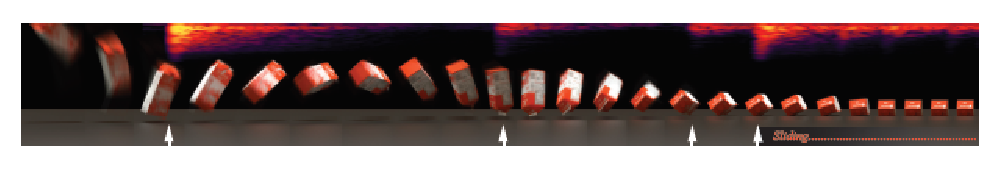
\includegraphics[width=15cm]{fig/chap2/IFA.eps}
	\caption{落下アニメーションの自動生成}
	\label{fig:IFA}
\end{figure}

\indent
キャラクタの口の動きと音声を合わせる,リップシンクも難しい課題となっている.
キャラクタの口の動きに合わせて後から音声を録音するアフレコは比較的容易であるが,音声から,その言葉を発している口元のアニメーションの生成は,言葉と口の形,そして発するタイミングと口の動きを合わせる必要があり,ひじょうに難易度が高い.
そこで,Edwardsら\cite{JALI}は,台詞が収録されている音源および台詞が記載されているテキストファイルを入力すると,その台詞を話している口元のアニメーション\ref{fig:JALI}を自動生成する手法を提案した.
本手法では,顎と唇のみを制御することにより,自然な口元のアニメーションを自動生成している.更に,後から表情を編集することが可能となっているため,最終的には自然な表情のアニメーションが完成する.
\begin{figure}[h]
	\centering
	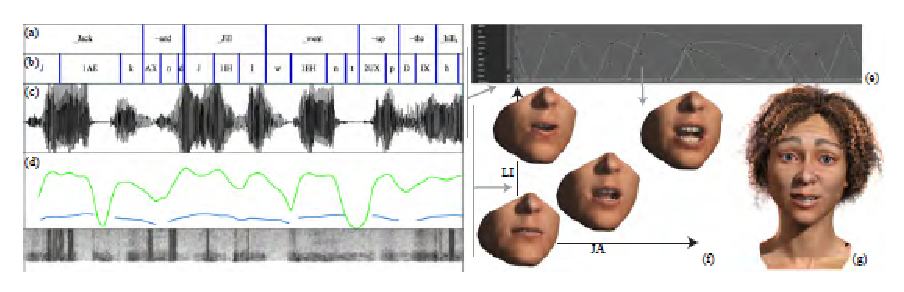
\includegraphics[width=15cm]{fig/chap2/JALI.eps}
	\caption{口元アニメーションの自動生成}
	\label{fig:JALI}
\end{figure}

\section{アニメーションから音を生成する研究}\label{sec:generate_sound}

\section{音とアニメーションを同期させる研究} \label{sec:synchronization}

\section{本研究との関連}\label{sec:compere}




%%%% 本研究のアプローチ
\chapter{提案手法} \label{chap:algorithm}
本章では提案手法を詳しく説明する.
まず,\secref{sec:flow}にて自動生成の大まかな流れを説明し,その後にそれぞれの工程について詳しく述べる.
\secref{sec:input}および\secref{sec:output}にて入出力について説明し,
\secref{sec:device}にて使用するデバイス,
\secref{sec:software}にて使用するソフトウェア,
\secref{sec:3Dmodel}にて使用する3Dモデルについて述べる.
\secref{sec:analysis}にてMIDIデータから音情報への変換方法,
\secref{sec:adapt}にて音情報のモーションへの適用方法を説明する.
そして最後に,\secref{sec:howto}にて実際にシステムを使用する際の,使用方法について言及する.

\section{自動生成の流れ} \label{sec:flow}
\figref{fig:flow}に,音源から吹奏アニメーションを自動生成する流れを示す.\\
\begin{figure}[!h]
	\centering
	\includegraphics[width=14cm]{fig/chap3/flow.eps}
	\caption{音源から吹奏アニメーションを自動生成する流れ}
	\label{fig:flow}
\end{figure}
\\
\indent
実際のアニメーション制作フローに沿わせるため,音源の生成は電子楽器を用いて行う.
次に,生成した音源を解析し,譜面データへ変換する.
そして,アニメーション生成と同時に音源を流すことにより,音源に合わせてキャラクタが動くアニメーションを自動生成する.

\section{入力} \label{sec:input}
入力する音源は,MIDI音源とする.
ここで,MIDI音源は,MIDIという信号を用いて発音する音源のことである.
一般的に使用されるmp3やwaveなどの形式とは異なり,中身が譜面データとなっているため,音の解析が比較的容易である.
なお,MIDIの仕様は文献\cite{midi}に詳しく記載されている.\\
\indent
このMIDI音源を生成する方法は,\secref{sec:device}および\secref{sec:software}で説明する.

\section{出力} \label{sec:output}
出力は,管楽器を演奏するキャラクタのアニメーションである.
今回対象とする管楽器は,トランペット,トロンボーンである.
この2本の楽器は,吹奏楽ではとくに目立つ楽器であり,また3Dモデルが入手しやすかったために選んだ.

\section{デバイス} \label{sec:device}
MIDI音源を生成するために,電子楽器であるウインドシンセサイザ「EWI5000」(\figref{fig:ewi})を使用する.
このウインドシンセサイザは,さまざまな楽器の音を再現することが可能である.
\begin{figure}[h]
	\centering
	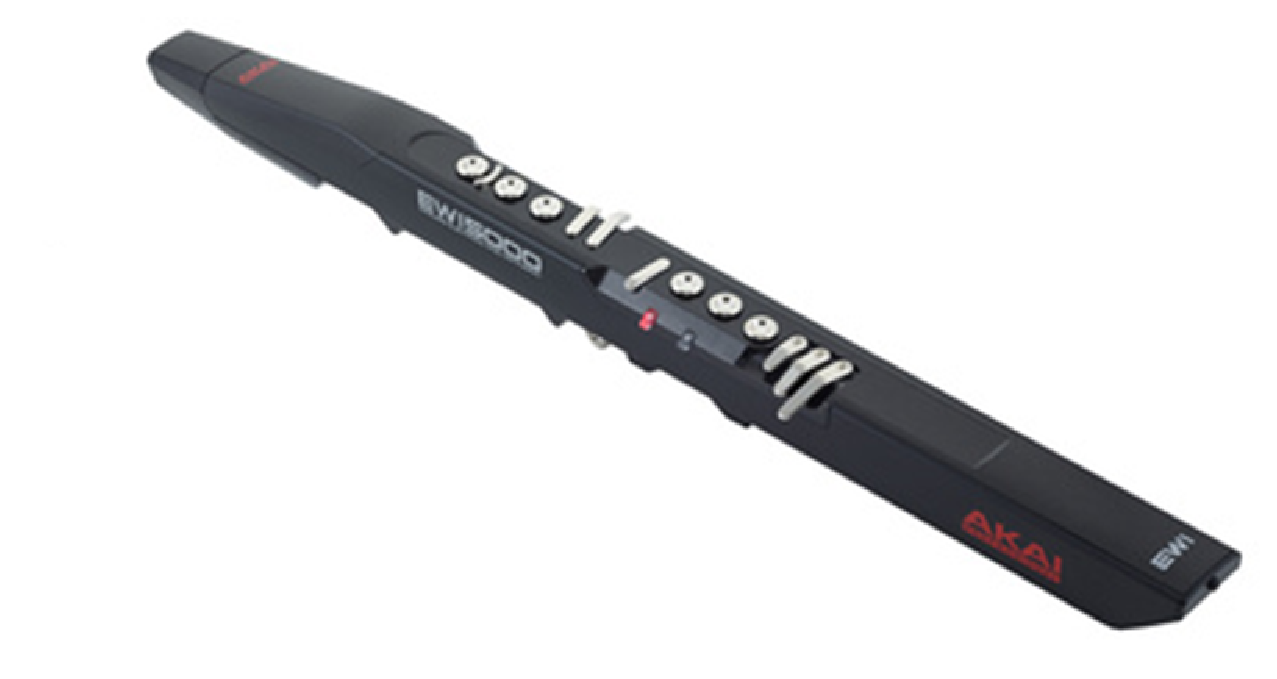
\includegraphics[width=10cm]{fig/chap3/ewi.eps}
	\caption{ウインドシンセサイザ「EWI5000」}
	\label{fig:ewi}
\end{figure}

\section{ソフトウェア} \label{sec:software}
\begin{figure}[h]
	\centering
	\includegraphics[width=10cm]{fig/chap3/domino.eps}
	\caption{MIDIシーケンスソフトウェア「domino」}
	\label{fig:domino}
\end{figure}
\secref{sec:device}で述べたウインドシンセサイザは,単音しか鳴らすことができないため,シングルチャンネルの音源しか生成することができない.
しかし,吹奏アニメーションを自動生成するためには,複数名で演奏しているマルチチャンネルの音源が必要となる.
そこで,ウインドシンセサイザで生成したMIDI音源を,フリーソフトウェアであるMIDIシーケンスソフトウェア「Domino」(\figref{fig:domino})\cite{domino}へ出力し,重ねて何度も録音することにより,マルチチャンネルの音源を生成する.\\
\indent
また,アニメーションの生成には,Epic Gamesより開発されたゲームエンジン,Unreal Engine\cite{ue4}を用いる.

\section{3Dモデル} \label{sec:3Dmodel}
使用する3Dモデルは,
ユニティちゃん(\subfigref{fig:model}{fig:unity}),トランペット(\subfigref{fig:model}{fig:tp}),トロンボーン(\subfigref{fig:model}{fig:tb})である.
それぞれ,\cite{unity},\cite{tp},\cite{tb}からダウンロードした.
なお,ユニティちゃんのライセンス条約は,webサイト\cite{license}にて確認済みである.
\begin{figure}[h]
	\centering
	\subcaptionbox{\textgt{ユニティちゃん}
		\label{fig:unity}}[0.75\linewidth]{
		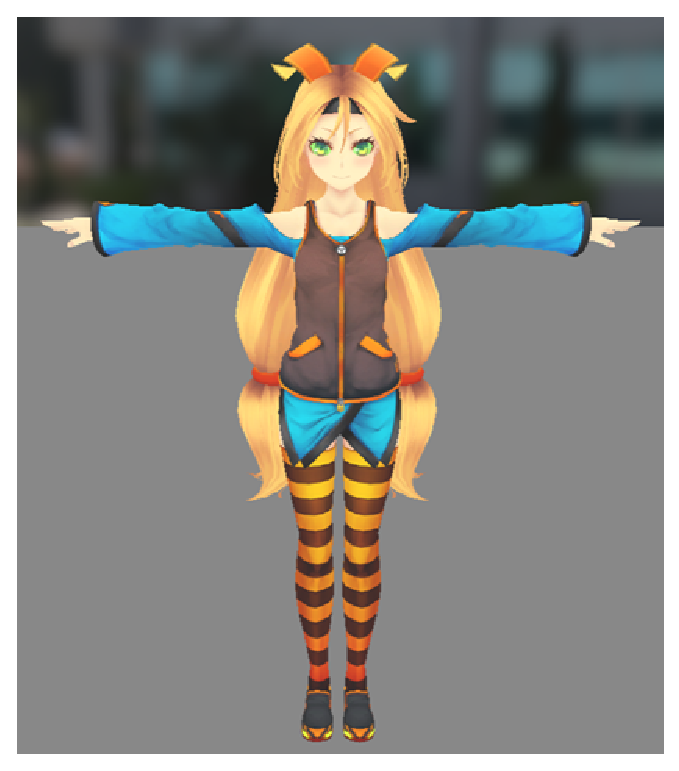
\includegraphics[height=7cm]{fig/chap3/unity.eps}}
	\subcaptionbox{\textgt{トランペット}
		\label{fig:tp}}{
		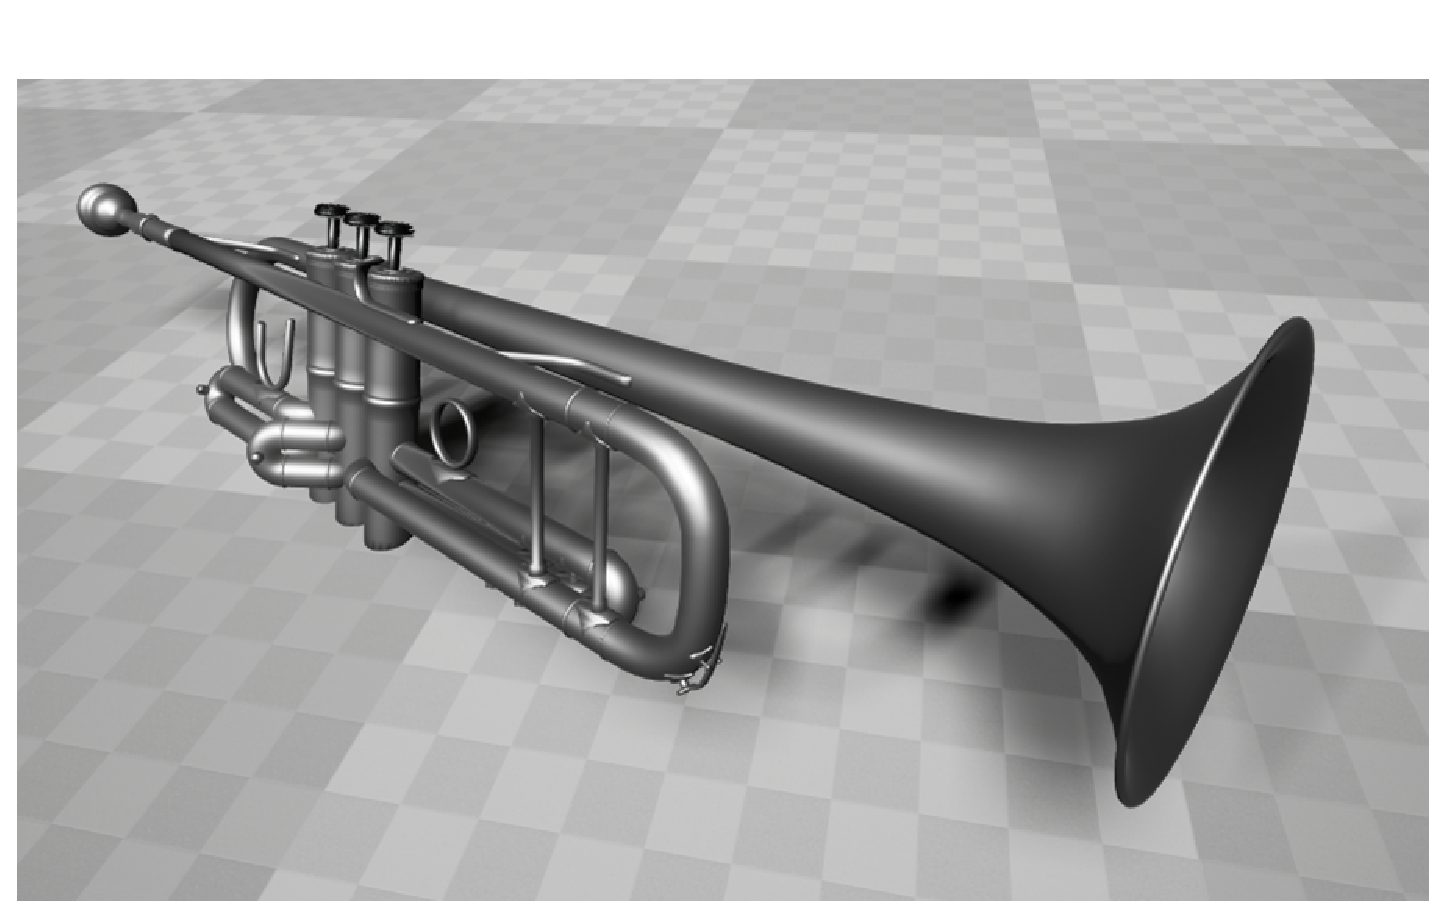
\includegraphics[width=6.5cm]{fig/chap3/tp.eps}}
	\subcaptionbox{\textgt{トロンボーン}
		\label{fig:tb}}{
		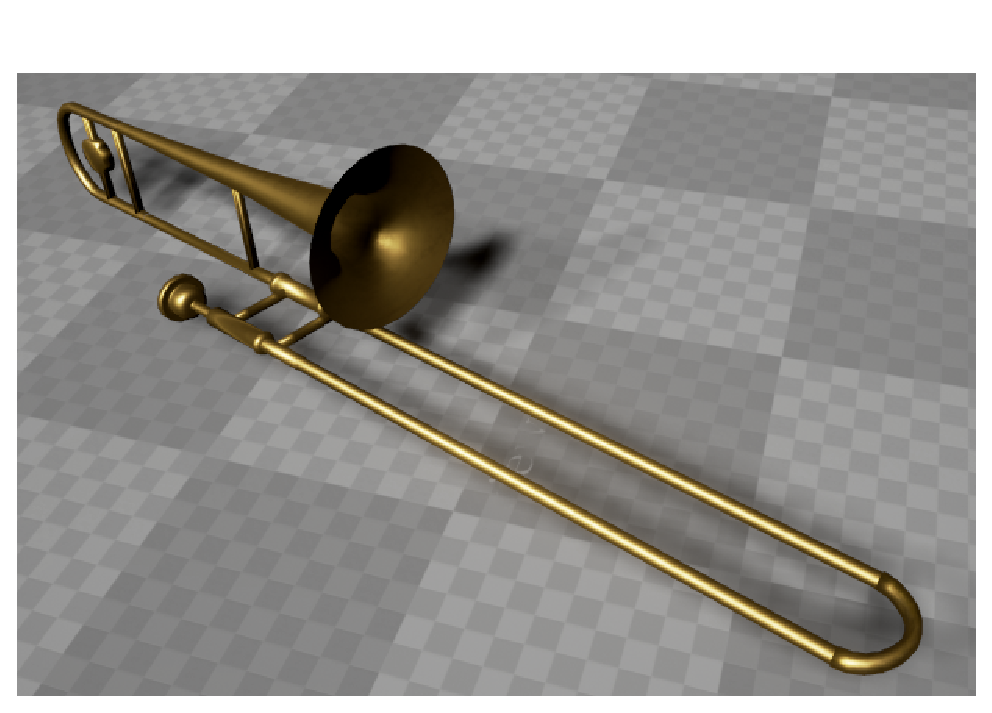
\includegraphics[width=7.5cm]{fig/chap3/tb.eps}}
	\caption{使用する3Dモデル}
	\label{fig:model}
\end{figure}
\newpage
\indent
ユニティちゃんは,主に以下の部位を制御する.
\begin{itemize}
	\item 右指(トランペット演奏時)
	\item 右腕(トロンボーン演奏時)
	\item 背
	\item 腰
	\item 両足
	\item 口元
\end{itemize}
\section{MIDIデータから音情報への変換} \label{sec:analysis}
MIDIは,チャンクとよばれるデータブロックから構成され,先頭にヘッダチャンク,その後にトラックチャンクが続く.
ヘッダチャンクには,チャンクタイプ,データ長さ,フォーマットタイプ,トラック数,タイムベース値という5つの値が格納されている.
ここで,タイムベース値とは,四分音符1つ分のクロック数を表す値であり,一般的には48から960までの自然数から,96の倍数が選ばれることが多い.
一方トラックチャンクには,チャンクタイプ,データ長,トラックイベントデータが格納されている.
提案手法では,トラック数,タイムベース値,トラックイベントデータを楽譜データに変換した後に,アニメーションに適用できる形へとさらに変更する.\\
\indent
まず,音に関する情報を楽譜データに変換する方法について説明する.
テンポ情報は,四分音符あたりの秒数($\mu$s)として格納されている.
音に関する情報は,トラックイベントデータとして,以下のように16進数で格納されている.\\

\hspace{10mm}9 0 4 8 6 4 8 1 7 0 8 0 4 8 0 0 8 3 6 0\\

この情報を2つずつペアにし,そこから音の種類と長さを取得する.
それぞれの数字から得られる情報は,以下の通りである.
\newpage
\begin{itemize}
	\item 90: ノートオン.このタイミングで音を鳴らすことを意味する.
	\item 48: 音の種類(48はドを意味する.対応表は次項に示す.)
	\item 64: 音の大きさ
	\item 81: 音を鳴らす長さ
	\item 70: 音を鳴らす長さ
	\item 90: ノートオフ.このタイミングで音を止めることを意味する.
	\item 48: 音の種類(48はドを意味する.)
	\item 00: 音の大きさ(音を止めているため,大きさはゼロとなる.)
	\item 83: 音を止める長さ
	\item 60: 音を止める長さ
\end{itemize}
\vspace{5mm}
音の長さは,以下のように取得する.ここでは,81 70を用いて説明する.
\begin{itemize}
	\item それぞれを2進数に変換する.\hspace{1mm}81: 1000 0001,70: 0111 0000
	\item それぞれの最上位ビットを取り除いて合成し,10進数に直す.\hspace{1mm}000 0001 111 0000 → 240
\end{itemize}
\vspace{5mm}
この例の場合,ドを240クロック分伸ばすことを意味する.以降,この値をデルタタイムとよぶ.
%デルタタイムを楽譜の情報に直すには,本節の冒頭で述べたタイムベース値を用いる.
最後に,このクロックを現実時間[s]に変換する.変換式は\eqref{eq:eq1}で表される.\\
\begin{equation}
\label{eq:eq1}
時間[s] = 
\frac {デルタタイム[ticks] × 60[seconds/minute]}{タイムベース値[ticks/beat] * テンポ[beats/minute]}
\end{equation}
\\
タイムベース値,テンポをそれぞれ仮に480,120とすると,例で示した音情報は,譜面情報に直した結果『ドを0.25秒伸ばし,0.5秒休む』ことを意味すると分かる.
\newpage
\section{音情報のモーションへの適用} \label{sec:adapt}
\subsection{指や腕,楽器のパーツへの適用}
楽器を演奏する様子をアニメーションで再現するには,キャラクタの指や腕を介して楽器のモデルを制御する必要がある.
トランペットはピストンの操作,トロンボーンはスライドの操作により音を変えることができ,ピストンは3箇所,スライドは止める場所が大きく分けて7箇所ある.
トランペットのピストン番号を,吹き口に近い方から1-3(\subfigref{fig:numbering}{fig:piston}),トロンボーンのスライドの位置を,吹き口に近い方から1-7(\subfigref{fig:numbering}{fig:slide})と表すと,MIDIデータと音,運指の対応は\tabref{tab:map}となる.
\begin{figure}[h]
	\centering
	\subcaptionbox{\textgt{ピストン番号}
		\label{fig:piston}}{
		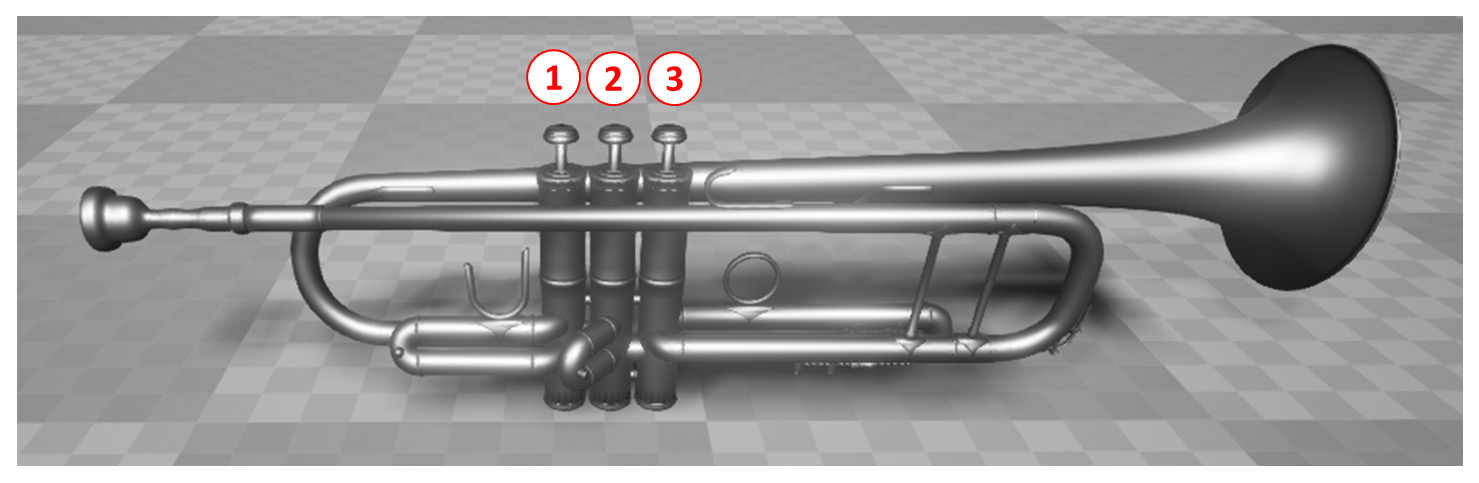
\includegraphics[width=10cm]{fig/chap3/tp_piston.eps}}
	\subcaptionbox{\textgt{スライドの位置番号}
		\label{fig:slide}}{
		\includegraphics[width=13cm]{fig/chap3/tb_slide.eps}}
	\caption{トランペットのピストンおよびトロンボーンのスライドの番号付け}
	\label{fig:numbering}
\end{figure}

\begin{table}[h]
	\centering
	\caption{MIDIデータと音,運指の対応}
	\begin{tabular}{|c|c|c|c|} \hline
		MIDIデータ & 音名(実音) & トランペット & トロンボーン \\ \hline \hline
		\vdots & \vdots & \vdots & \vdots \\ \hline
		39 & A(ラ,442Hz) & 2 & 2 \\ \hline
		3b & B(シ) & 1・2・3 & 4 \\ \hline
		3c & C(ド) & 1・3 & 3 \\ \hline
		3e & D(レ) & 1・2 & 1 \\ \hline
		40 & E(ミ) & 2 & 2 \\ \hline
		41 & F(ファ) & 0 & 1 \\ \hline
		43 & G(ソ) & 1・2 & 2 \\ \hline
		45 & A(ラ) & 2 & 2 \\ \hline
		\vdots & \vdots & \vdots & \vdots \\ \hline
	\end{tabular}
	\label{tab:map}
\end{table}
\newpage
\secref{sec:analysis}で例として挙げた,『ドを0.25秒伸ばし,0.5秒休む』という譜形を演奏する場合,トランペットの場合は,1番と3番を0.25秒間押し続け,その後0.5秒間は休みのためそのまま,トロンボーンの場合は,スライドを3番まで移動させ,そのまま0.25秒間維持,その後0.5秒間は休みのためそのまま,という表現方法となる.\\

\newpage
\subsection{口元のメッシュへの適用}
\indent
金管楽器を演奏する際,高音域の演奏時は,低音域に比べて口元が緊張する.
緊張の程度には個人差があるが,本論文では,高音演奏時と低音演奏時の口元の違いを\figref{fig:mouth}のように,口の引き具合で表す.
\vspace{-2mm}
\begin{figure}[H]
	\centering
	\subcaptionbox{\textgt{低音域演奏時}
		\label{fig:low}}[0.45\linewidth]{
		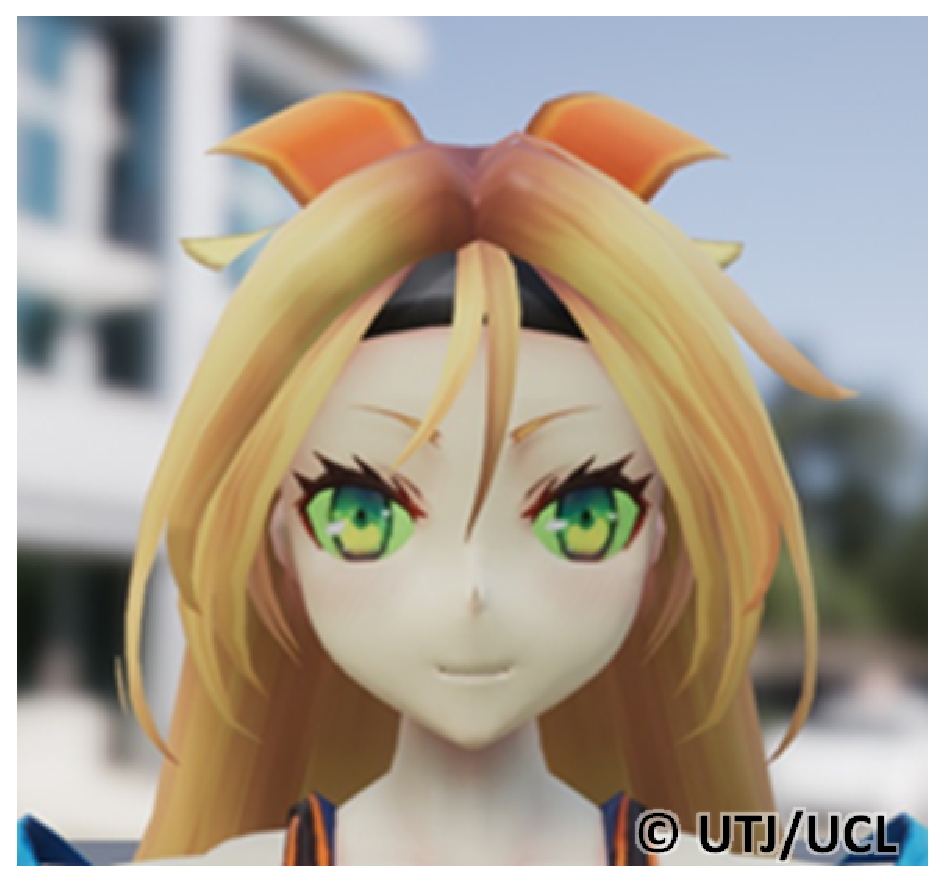
\includegraphics[width=6cm]{fig/chap3/low.eps}}
	\subcaptionbox{\textgt{高音域演奏時}
		\label{fig:high}}[0.45\linewidth]{
		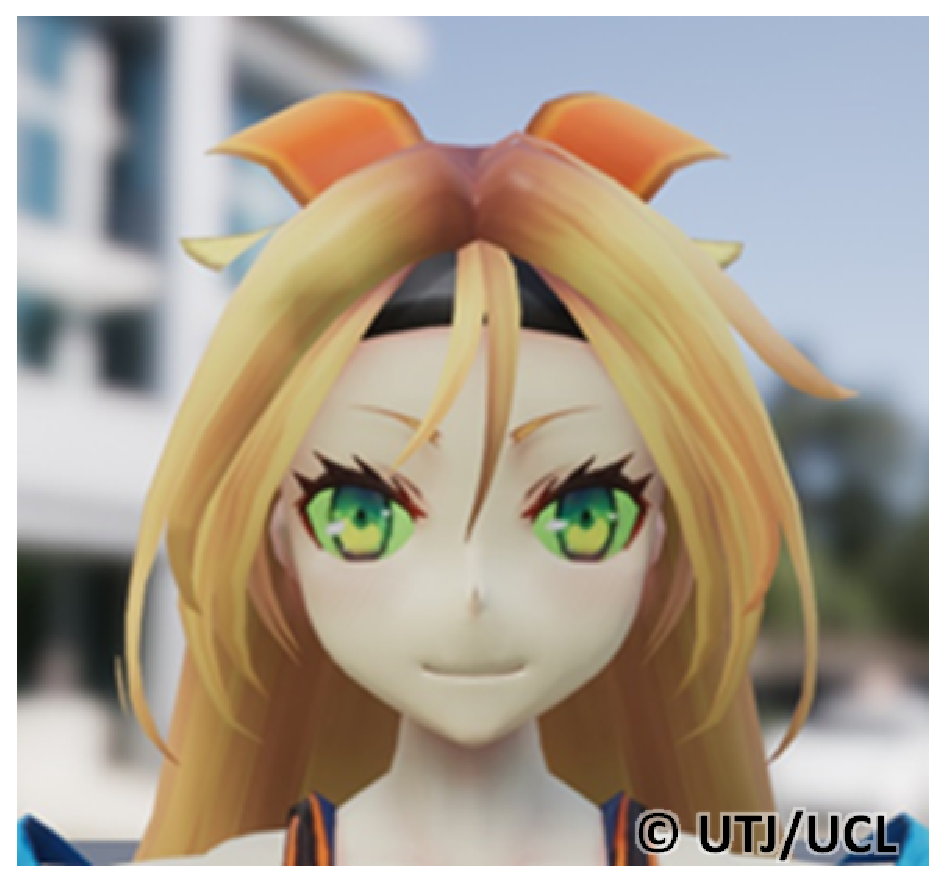
\includegraphics[width=6cm]{fig/chap3/high.eps}}
	\caption{音域による口元の変化}
	\label{fig:mouth}
\end{figure}
\indent
休みが一定の時間以上続く場合,演奏者は息継ぎを行う.息継ぎのタイミングには個人差があり,演奏しているフレーズによっても異なるが,提案手法では息継ぎのタイミングを以下の3パターンに分ける.
\begin{itemize}
	\item 休みが0.5拍以上~1拍未満: 休みの間,息継ぎのモーションを行う.
	\item 休みが1拍以上~2拍未満: 最後の1拍で息継ぎのモーションを行う.
	\item 休みが2拍以上: 最後の2拍間で,息継ぎの予備モーションおよび息継ぎのモーションを行う.
\end{itemize}

息継ぎのモーションを行うときに,口元を\figref{fig:breath_mouth}のように変形させる.
その他のモーションについては次項で述べる.\\
\vspace{-2mm}
\begin{figure}[!h]
	\centering
	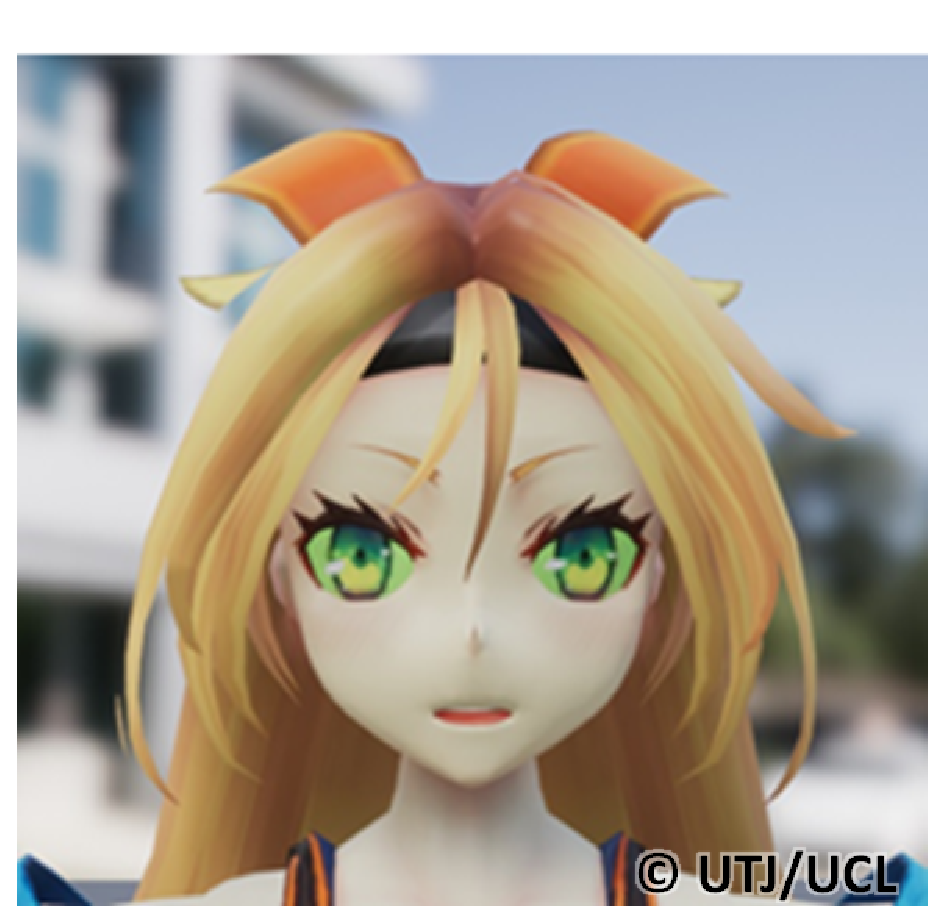
\includegraphics[width=6cm]{fig/chap3/breath.eps}
	\caption{息継ぎをするときの口元}
	\label{fig:breath_mouth}
\end{figure}
\newpage
\subsection{その他の部位への適用}
\indent
息継ぎをするときは口元だけでなく,上半身も動く.
そこで,前項で述べたタイミングで,
息継ぎのモーション\subfigref{fig:breath_motion}{fig:breath_up},
息継ぎの予備モーション\subfigref{fig:breath_motion}{fig:breath_down}を行う.
なお,比較対象として通常の直立状態を\subfigref{fig:breath_motion}{fig:breath_default}に示す.差が分かりづらい場合は,楽器と床の端との位置関係を見てほしい.\\
\begin{figure}[!h]
	\centering
	\subcaptionbox{\textgt{息継ぎのモーションの最中}
		\label{fig:breath_up}}[0.45\linewidth]{
		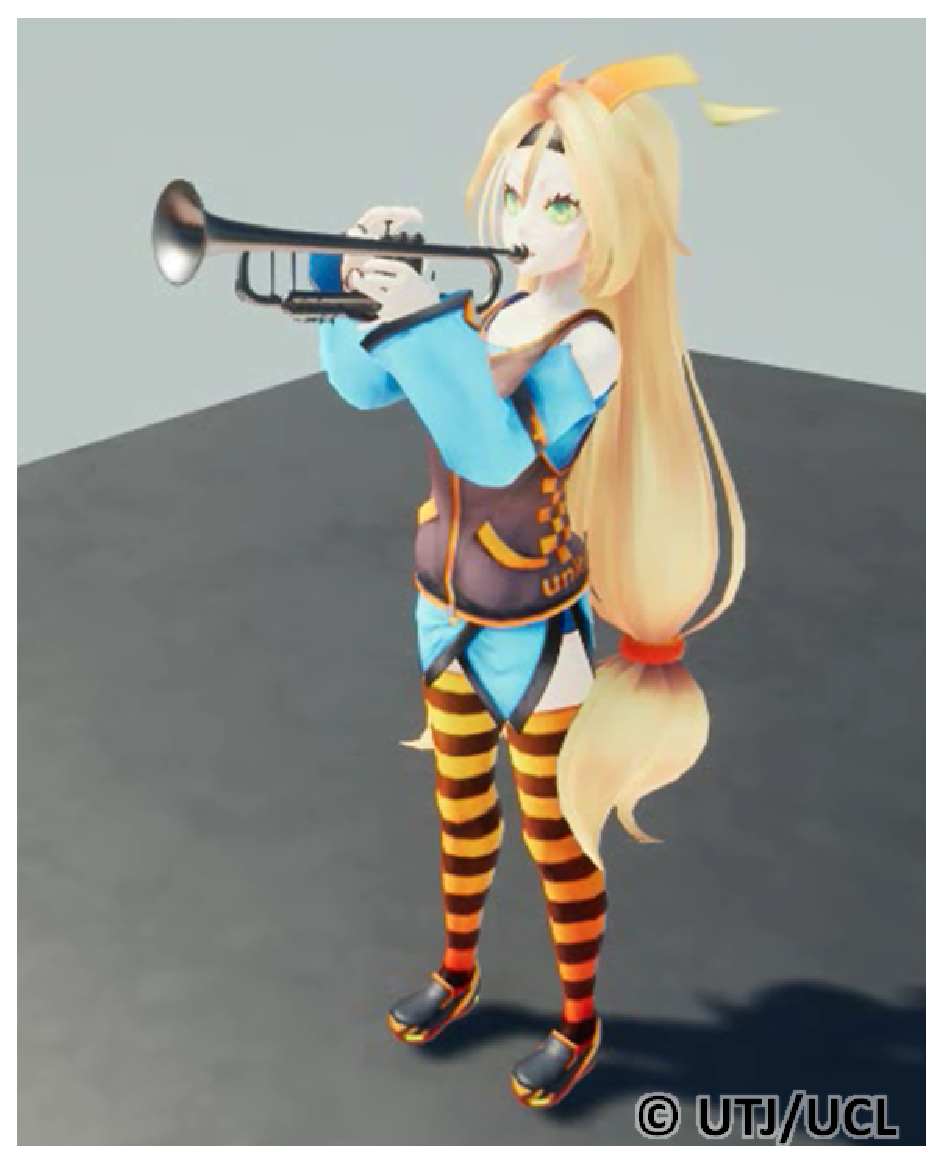
\includegraphics[width=6cm]{fig/chap3/up.eps}}
	\subcaptionbox{\textgt{息継ぎの予備モーションの最中}
		\label{fig:breath_down}}[0.45\linewidth]{
		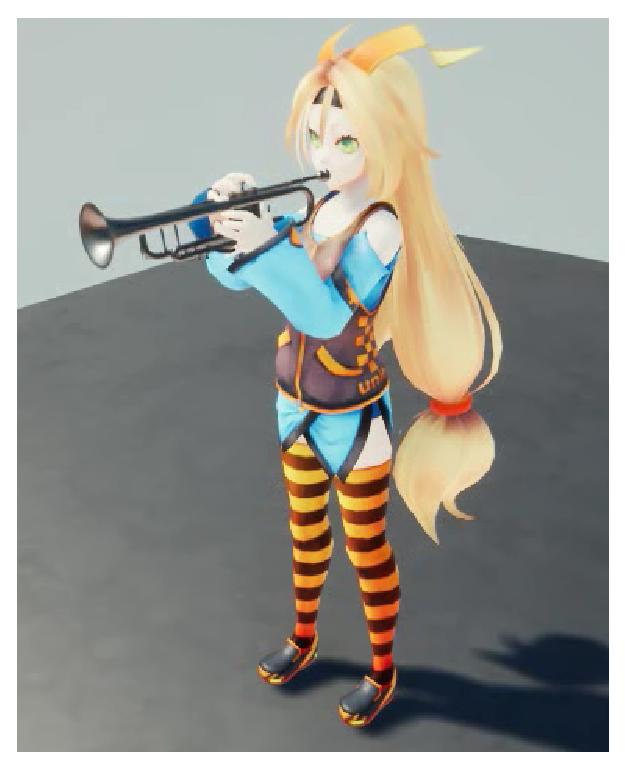
\includegraphics[width=6cm]{fig/chap3/down.eps}}
	\subcaptionbox{\textgt{通常の直立状態}
		\label{fig:breath_default}}[0.45\linewidth]{
		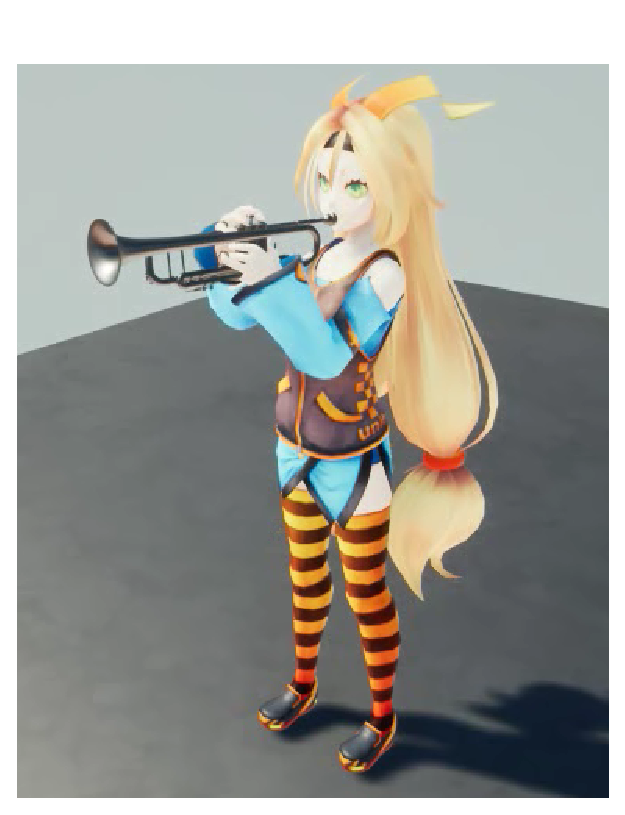
\includegraphics[width=6cm]{fig/chap3/default.eps}}
	\caption{息継ぎ時のモーション}
	\label{fig:breath_motion}
\vspace{10mm}
\end{figure}
\newpage
\indent
息継ぎ時以外にも演奏者は動く.
例えば,任意のタイミングで重心を移動させたり,テンポに合わせて身体や楽器を上下に揺らす.
しかし実際,演奏時の動きには個人差があるため,モーションの大きさを調節するためのパラメタを指定することによる個人差の表現が可能となっている.
%現在はランダムでパラメタが設定される仕様となっている.
アンサンブルアニメーションを自動生成する際は,全員に異なるパラメタをランダムで割り当てることにより,個人差を表現する.
ここで,アンサンブルとは複数名で演奏することを意味し,一般的には少人数で演奏することをさす.
アンサンブルには指揮者が存在しないため,曲の始まりは,リードを担当する演奏者が楽器や身体で合図をする.
なお,重心移動や合図のモーションは,同研究室学士4年の武内が担当した.
%音情報から一意に定義可能なモーションは堀井.\\

\section{提案手法の使用方法} \label{sec:howto}
提案手法を用いてアニメーションを自動生成する際は,以下の順序が必要となる.
ここで,キャラクタや楽器のモデルは,あらかじめセッティングされているものとする.
\begin{enumerate}
	\item MIDI音源の作成
	\item 音源データの相対パスをソースコードに記載し,コンパイル
	\item Unreal Engineを起動
	\item 1.で生成した音源をBGMとして設定
	\item 再生
	\item 結果の確認および修正
\end{enumerate}\par
手順4.について,本来ならMIDI音源を解析すると同時に音を流すべきであるが,現在の実装ではそれが不可能となっているため,解析する音源とは別に,流す音源として新たに設定する必要がある.
また,このとき音のずれが生じる場合がある.その場合は,音源を流すタイミングの調節が必要となるが,一度調節をするだけでアニメーションと音は完全に同期する.
%%%% アルゴリズム
\chapter{結果と評価}
\label{chap:results}
本章では,3章で紹介した手法によって自動生成した吹奏アニメーションについて記述する.
\secref{sec:system}では仕様したPCやシステムの仕様を述べ,
\secref{sec:result}では自動生成した吹奏アニメーションのキャプチャリング画像を示す.
そして\secref{sec:review}では自動生成結果を実際の演奏シーンや既存の吹奏アニメーションと比較することにより,提案手法を評価する.

\section{実行環境} \label{sec:system}
事前にUnreal Engineにて専用のプロジェクトを作成し,モーションのデータが記載されているUnreal Engine専用のファイルをインポートする.
そして,キャラクタと,それぞれが演奏する楽器を\figref{fig:ue4}のようにセッティングする.
なお,最初にインポートするUnreal Engine専用のファイルには,キャラクタの姿勢データも存在するため,
キャラクタの姿勢のセッティングは容易にできる.\\
\indent
実行環境は\tabref{tab:pc}の通りである.
\begin{figure}[h]
	\centering
	\includegraphics[width=14cm]{fig/chap4/ue4.eps}
	\caption{Unreal Engineの初期設定}
	\label{fig:ue4}
\end{figure}

\begin{table}[htbp] 
	\begin{center}
		\caption{実行環境}
		\label{tab:pc}
		\begin{tabular}{|l|c|}
			\hline
			OS & Windows10 64bit \\ \hline
			CPU & Intel\textregistered Core\textsuperscript{TM}i7-3930K \\ \hline
			RAM & 32.00GB\\ \hline
			言語 & c++\\ \hline
		\end{tabular}
	\end{center}
\end{table}

\section{アニメーション生成結果} \label{sec:result}
本研究で作成したアニメーションは,主に少人数編成であるアンサンブルアニメーションである.
以下では,トランペット奏者2名で演奏するアニメーションのキャプチャリング画像と,
トランペット奏者2名,トロンボーン奏者2名の計4名で演奏するアニメーションのキャプチャリング画像を示す.
以下,それぞれについて制御している口元やボーンの制御について説明するが,
前者のアニメーションは口元や指元がズームインされているシーンであるため,主に口元や指元のボーンの制御について,
後者のアニメーションは全体を俯瞰しているシーンであるため,主に指元以外のボーンの制御について述べる.\\
\indent
\figref{anim1}は,トランペット奏者2名の基本姿勢である.
\begin{figure}[h]
	\centering
	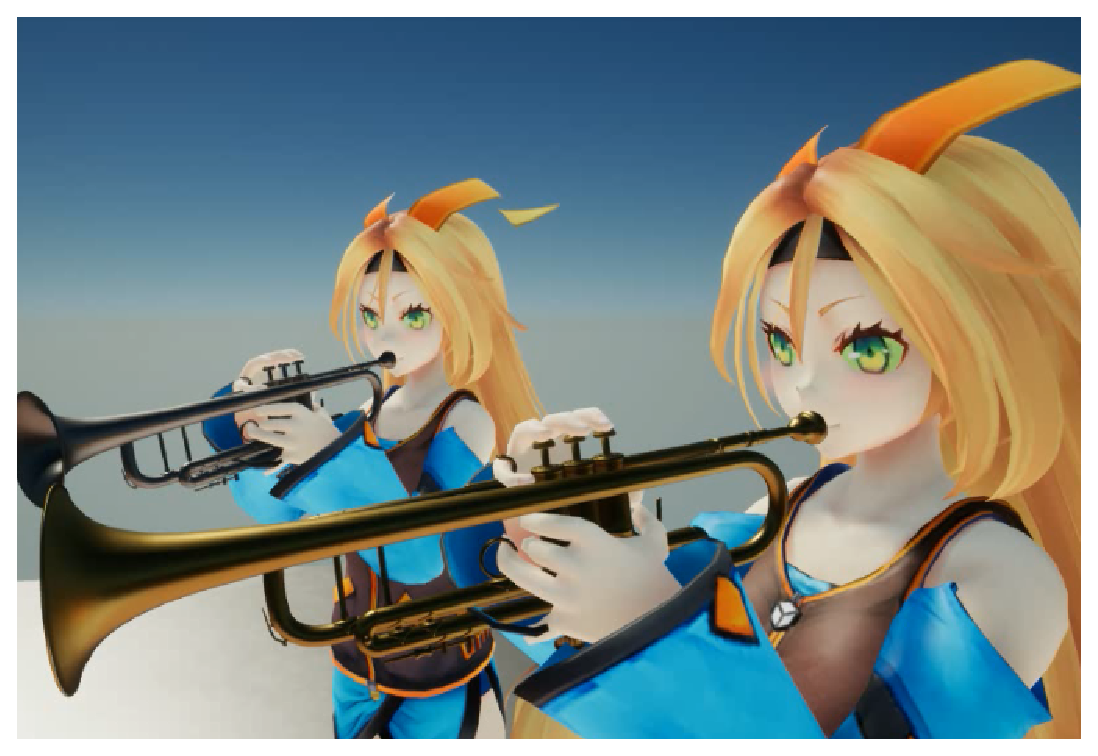
\includegraphics[width=10cm]{fig/chap4/anim1.eps}
	\caption{トランペット奏者2名の基本姿勢}
	\label{fig:anim1}
\end{figure}
音を鳴らすタイミングで,演奏者は\figref{anim1_finger}のように,指でトランペットのピストンを押す動作をする.
\begin{figure}[h]
	\centering
	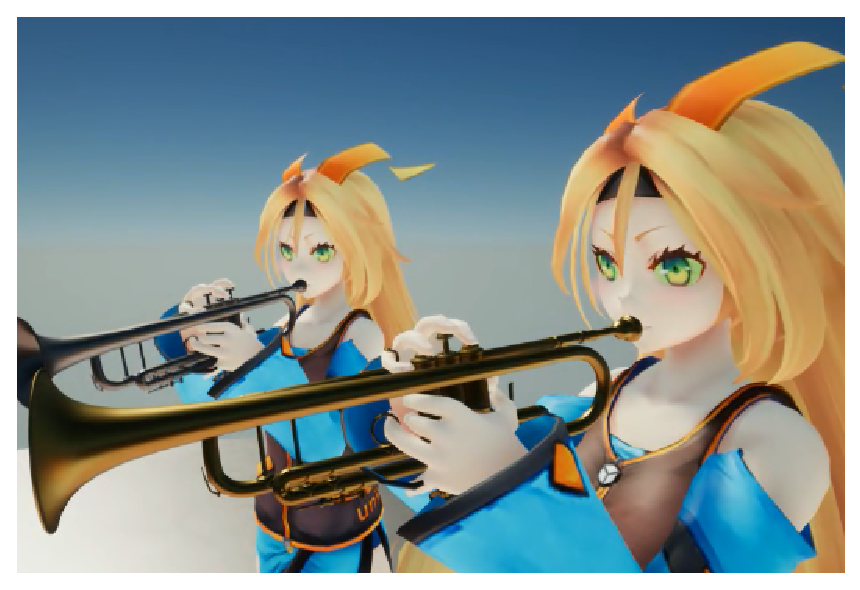
\includegraphics[width=10cm]{fig/chap4/anim1_finger.eps}
	\caption{トランペット奏者2名がピストンを押す姿勢}
	\label{fig:anim1_finger}
\end{figure}


\section{評価} \label{sec:review}

\subsection{実際の演奏シーンとの比較による評価}

\begin{figure}[t]
	\centering
	\subcaptionbox{\textgt{吹奏楽・オーケストラ経験者の回答}
		\label{fig:unity}}[0.75\linewidth]{
		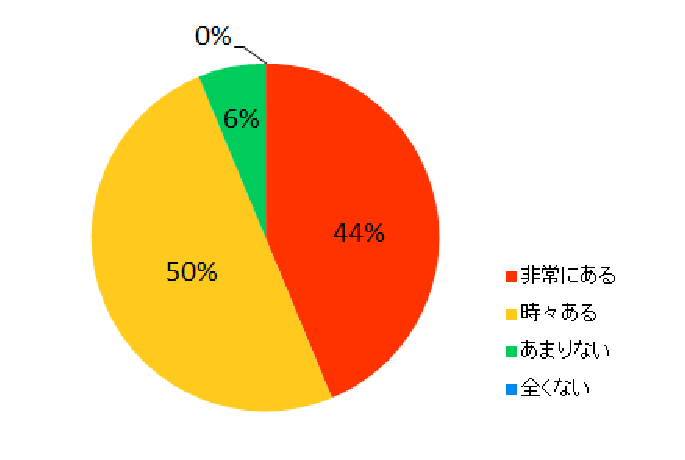
\includegraphics[height=7cm]{fig/chap1/Q1-1.eps}}
	\subcaptionbox{\textgt{吹奏楽・オーケストラ未経験者の回答}
		\label{fig:tp}}[0.6\linewidth]{
		\includegraphics[height=5.5cm]{fig/chap1/Q1-2.eps}}
	\caption{演奏アニメーションが不自然であると感じることがあるかどうか}
	\label{fig:model}
\end{figure}

\subsection{既存のアニメーションとの比較による評価}

\subsection{アンサンブルアニメーションの評価}

\subsection{システムの有用性の予想}
%%%% 結果と評価
\chapter{結論}
\label{chap:conclusion}
本章では本論文の結論を述べ,今後の課題に言及する.

\section{まとめ}

\section{今後の課題}

\subsection{表情の豊かさの向上}

\subsection{モーションの質と種類の向上}

\subsection{モーションと音の関連付け}

\subsection{楽器の種類および演奏者の増加}
%%%% 謝辞
\chapter*{謝辞}
\label{chap:thanks}
%
\addcontentsline{toc}{chapter}{謝辞} % 目次へ追加
%
本論文の執筆にあたり,ひじょうに多くのアドバイスを頂いたばかりでなく,さまざまな相談も聞いていただきました,慶應義塾大学理工学部情報工学科の藤代一成教授に深く感謝いたします.
特に,修士1年生の途中で研究テーマを変更するか否か迷っていた際に,多大な後押しをしていただきました.
藤代教授の後押しがあったからこそ,後悔のない研究室生活を送ることができました.
藤代研究室の一員として受け入れていただけたことを,改めて嬉しく思います.
本当にありがとうございました.\\
\par
本論文の執筆にあたり,貴重なご意見を頂きました,慶應義塾大学理工学部情報工学科の斎藤英雄教授,杉本麻樹准教授,杉浦裕太助教に深く感謝いたします.
お陰様で,広い視野を持って本論文を執筆することができました.\\
\par
本研究を進めるにあたり,実装面において多くのアドバイスを頂いただけでなく,コンピュータグラフィクス分野におけるさまざまな課題に出会う機会や,実際に業務に携わる機会を頂きました,株式会社デジタル・フロンティア開発部の皆様に深く感謝いたします.\\
\par
本研究を進めるにあたり,時には楽しく話し合い,時には真面目に議論を行い,共に助け合った研究室の皆様に深く感謝いたします.
特に,共同で研究を進めてくれた研究室学士4年の武内氏は,吹奏楽の経験がないにも関わらず何度もディスカッションを重ね,私のさまざまな要求に答えてくれました.
また同期の皆様は,時には優しく,時には厳しく,私の研究室生活を支えてくれました.このメンバーでなければ,ここまで楽しく充実した研究室生活を送ることはできませんでした.\\
\par
最後に,本研究の評価アンケートにご協力いただきました,藤代研究室の皆様,株式会社デジタル・フロンティア開発部の皆様,お茶の水女子大学伊藤研究室の皆様,株式会社スクウェア・エニックス2018年新卒の皆様,東京個別指導学院高円寺教室の講師の皆様,應援指導部の皆様,慶應義塾大学塾生会館受付アルバイトの皆様,高校時代のクラスメイトの皆様に,厚く御礼申し上げます.

\renewcommand{\refname}{���J����}	

\begin{thebibliography}{55}
\addcontentsline{toc}{chapter}{���J����}% �lj�

\bibitem[31]{Kimura11}
Kimura, H., Asano, A., Fujishiro, I., Nakatani, A., and Watanabe, H.:\,``True 3D Display,"
{\it ACM SIGGRAPH 2011 Emerging Technologies},
August 2011,
abstract available in Full Conference DVD-ROM.

\bibitem[32]{Nakatani11}
���J �����C���� �ꐬ�C�ؑ� �G�сC��� ���F
�u3�����f�B�X�v���C�̂��߂̓����_��̒��o�Ɋւ���V�~�����[�V�����]���v�C
Visual Computing/GCAD�����V���|�W�E��2011DVD�\�e�W�CNo.\,30�C
2011�N6���D

\bibitem[33]{Nakatani11_2}
���J �����C���� �ꐬ�C��� �`�v�F
�u�R�x�`��ɂ�����ϐ�ʂ𐧌䂷��T�[�t�F�X�L�q�q�̒�āv�C
�|�p�Ȋw��_�����CVolume\,10�CNo.\,2�C 
pp.\,79-86�C
2011�N6���D

\end{thebibliography}
\renewcommand{\refname}{参考文献}	
%
\begin{thebibliography}{55}
\addcontentsline{toc}{chapter}{参考文献}% 追加
%
\bibitem{Lee}H. C. Lee and I. K. Lee,
 ``Automatic Synchronization of Background Music and Motion in Computer Animation,"
 \textit{Computer Graphics Forum,} Vol. 24, No. 3, pp. 353-361, September 2005.

\bibitem{IFA}T. R. Langlois and D. L. James,
 ``Inverse-Foley Animation: Synchronizing Rigid-body Motions to Sound,"
  \textit{ACM Transactions on Graphics,} Vol. 33, No. 4, Article No. 44, pp. 44:1-44:11, July 2014.

\bibitem{JALI}P. Edwards, C. Landreth, E. Fiume, and K. Singh,
 ``JALI An Animator-Centric Viseme Model for Expressive Lip Synchronization,"
  \textit{ACM Transactions on Graphics,} Vol. 35, No. 4, pp. 127:1-127:11, July 2016.

\bibitem{piano}Y. Zhu, A. S. Ramakrishnan, B. Hamann, and M. Neff,
 ``A System for Automatic Animation of Piano Performances,"
  in \textit{Proceedings of Computer Animation and Virtual Worlds,} Vol. 24, No. 5, pp. 445-457, September 2012.

\bibitem{domino}http://takabosoft.com/domino
(最終アクセス日: 2018/02/05).

\bibitem{tf3dm}http://tf3dm.com/
(最終アクセス日: 2018/02/05).

\bibitem{3dexport}https://jp.3dexport.com/
(最終アクセス日: 2018/02/05).

\bibitem{CG-ARTS}CG-ARTS, ``音を描き出す夢の実現," 最終アクセス:2018年2月5日. 
[Online]https://www.cgarts.or.jp/report/rep\_kr/rep0901.html

\end{thebibliography}

\end{document}


\end{thebibliography}

%\renewcommand{\refname}{参考文献}
%\bibliographystyle{macros/IEEEtran}
%\bibliography{thesis}

%%%% 付録 A
%\newpage
%\pagenumbering{arabic}           % アラビア数字のページナンバリング
%\def\thepage{A--\arabic{page}}		% ページ数をA-1. A-2,... と表示
%\appendix	
%\chapter*{付録}
\label{chap:appendix}
\addcontentsline{toc}{chapter}{付録} % 目次へ追加
\renewcommand{\thepage}{A-\roman{page}}


\end{document}

